\chapter*{Discussion}
\label{ch:discussion}

An interesting aspect of the explainability analysis is the visualization of the results.
The \textbf{left section} of the graph in Figure~\ref{fig:expl} displays the predicted probabilities for each class. In the \textbf{center section}
feature importances are ranked from most to least relevant and divided into two groups: on the right
features with a positive influence on the predicted label; on the left, those with a negative influence that suggest the model should consider other classes.
The \textbf{right section} of the graph highlights the values of the most important
features, using bright colors to indicate features with a positive influence on the prediction.

\begin{figure}[H]
    \centering
    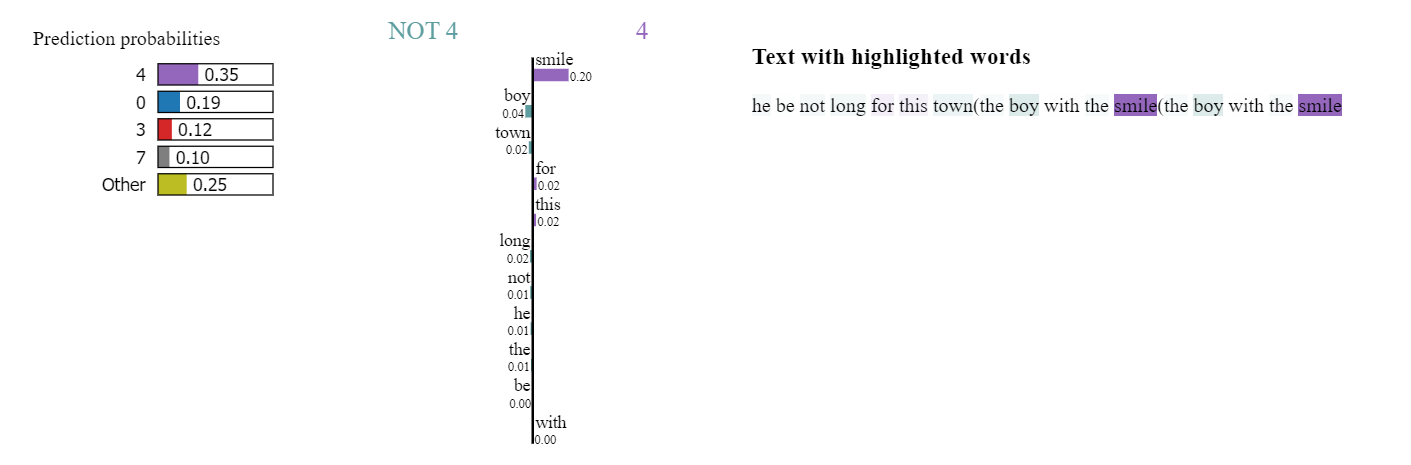
\includegraphics[scale= 0.55]{pictures/expl.png}
    \caption{Explainability - visualization}
    \label{fig:expl}
\end{figure}

The figure above illustrates a prediction where the model assigned the label \textit{joy} to the stanza under analysis, but the correct label, assigned by the ALBERT model (as mentioned in the \textit{Methods} section), was \textit{sadness}.
However, the word \textit{smile}, which is brighty highlighted, intuitively suggests that \textit{joy} might be a more plausible class for this stanza, even one that ALBERT could reasonably assign. 
This observation raises a critical issue: the transfer learning approach used to create the ground truth appears to have some limitations; in some instances the SVC model assigns a label that seems more contextually appropriate for the stanza, 
yet it differs from the supposedly correct label provided by ALBERT.\\

This phenomenon may also explain the results presented in the figures from the
previous chapter.
However, it is not the only plausible explanation; notably, the poor performance
could be attributed to a general overlap of features.
By applying a filter to exclude the most common words, it's possible that the
remaining words carry less ambiguous emotional meanings, and are easier to interpret.
% TODO quote figures

